\documentclass{paper}

%% [lingua] definizione della/e lingua/e; la lingua di default del documento è sempre l'*ultima*
\usepackage[english,italian]{babel}
\usepackage[utf8]{inputenc}
\usepackage[T1]{fontenc}

%% [biblatex] introduzione pacchetti utili per BibLaTeX
\usepackage[babel]{csquotes}
\usepackage[babel=hyphen,hyperref,backend=biber]{biblatex}

\addbibresource{bibliografia.bib}

%% [geometria] stabilisco i margini
\usepackage[letterpaper]{geometry}
\geometry{verbose,lmargin=3cm,rmargin=3cm}

%% [immagini]
\usepackage{float}
\usepackage{graphicx}

%% [math]
\usepackage{siunitx}

%% [links] opzioni hyperref
\usepackage[unicode=true,bookmarks=true,bookmarksnumbered=false,bookmarksopen=false,breaklinks=true,pdfborder={0 0 1},backref=false,colorlinks=false]{hyperref}
\hypersetup{pdfauthor={Francesco de Virgilio}}

%% [notes] double columns notes
\usepackage[noeledmac]{ledmac}
\foottwocolX{A}

\begin{document}

%%%%%%%%%%%%%%%%%%%%%%%%%%%%%%%%%%%%%%%%%%%%%%%%%%%%%%%%%%%%%%%%%%%%%%%%%%%%%%%%
% CORREZIONI DI STILE %
%%%%%%%%%%%%%%%%%%%%%%%%%%%%%%%%%%%%%%%%%%%%%%%%%%%%%%%%%%%%%%%%%%%%%%%%%%%%%%%%

%% aggiunge una virgola tra Autore e anno nello stile citazione authoryear
\renewcommand{\nameyeardelim}{, } % this doesn't work anymore

%% sostituisce le parentesi tonde dell'anno di pubblicazione con "niente"
\renewcommand{\bibleftparen}{}
\renewcommand{\bibrightparen}{}

%% separa gli elementi della citazione con una virgola anzichè i punti
\renewcommand*{\newunitpunct}{\addcomma\space}

%% rende corsivo il titolo dell'articolo
\DeclareFieldFormat[article]{title}{\mkbibemph{#1}}

%% aggiunge "«»" al nome del giornale di pubblicazione, e fa seguire da una virgola
\DeclareFieldFormat{journaltitle}{\guillemotleft{#1}\guillemotright ,}
\DeclareFieldFormat{pages}{{#1}}

%%%%%%%%%%%%%%%%%%%%%%%%%%%%%%%%%%%%%%%%%%%%%%%%%%%%%%%%%%%%%%%%%%%%%%%%%%%%%%%%
% FINE CORREZIONI DI STILE %
%%%%%%%%%%%%%%%%%%%%%%%%%%%%%%%%%%%%%%%%%%%%%%%%%%%%%%%%%%%%%%%%%%%%%%%%%%%%%%%%

\title{WebGIS e divulgazione del dato archeologico con software open source}

\subtitle{Il progetto ``Siponto Aperta''}

% TODO: fix authors
\author{
    \large{Patrizia Albrizio\thanks{Laureanda in Archeologia}}
    \and
    \large{Francesco de Virgilio\thanks{\protect\href{mailto:francesco.devirgilio@openoia.org}{francesco.devirgilio@openoia.org}, laureando in Scienza e Tecnologia per la Diagnostica e Conservazione dei Beni Culturali}}
    \and
    \large{Ginevra Panzarino\thanks{Specializzanda in Archeologia}}
    \and
    \large{Enrica Zambetta\thanks{Specialista in Archeologia}}
}

\institution{O.I.A. --- Open Idea for Archaeology}

\date{Marzo 2013}
\maketitle

% TODO: fix multilanguage abstract
\begin{abstract}
IT abstract --- TODO\\

This paper shows how a set of open source tools, raging from CSS templates to JavaScript libraries, from PHP interfaces to PostGIS and MySQL databases, can be used to create a complete environment for both touristic and enhanced view of archaeological data.

During this experience various frontend tools have been analyzed and compared, and a some of them have been chosen to create a touristic purposed archaeological website, www.sipontoaperta.it, and the corresponding data management interface with on-request only access; in this setup the "stratigraphic unit" approach to data management has been mixed with "single context record"-based tools and spatial-enabled database plus Python scripts to obtain a full featured (albeit user friendly) webGIS.

The work also presents for the first time in literature a successful stratigraphic unit data import into the ARK platform, and an OpenLayer plus Pannellum setup to create the first 360 degree immersive photographic webtour documented on an archaeological site.

To increase the attractiveness and the competitiveness of the website, 3D laser-scanned reconstructions have been created, exported using well documented formats and embedded in the webGIS using open source JavaScript tools.
\end{abstract}

\begin{keywords}
    webGIS, ARK, OpenLayers, 3D models, geodatabase
\end{keywords}

NOTA BENE\\
Questo paper è una bozza e necessita ulteriori modifiche. Ci scusiamo per averlo presentato ancora incompleto, è stato difficile per noi realizzarlo entro la deadline fissata. Nello specifico, occorre inserire altre voci in bibliografia e ulteriori immagini che mostrino altre caratteristiche del prodotto realizzato. Ci scusiamo per questo, cercheremo di provvedere al più presto a colmare le lacune con una versione aggiornata del presente paper.

\pagebreak{}

\section{Il caso di studio}

    Siponto (Manfredonia -- Foggia) è un'antica colonia romana dedotta nel II sec. a.C., precoce diocesi della \emph{II regio Apulia et Calabria} e fiorente porto sull'Adriatico fino all'epoca dell'abbandono, decretato dal sovrano svevo Manfredi nel 1263. 

    L'indagine sulla città si inserisce nell'ambito del programma di ricerca su \emph{Siponto. Una città portuale abbandonata}, realizzato grazie alla collaborazione istituzionale con diversi enti, quali il Ministero dei Beni Culturali attraverso la Soprintendenza dei Beni Archeologici della Puglia, la provincia di Foggia con il Museo del Territorio, l'Università degli Studi di Bari --- Aldo Moro (Dipartimento di Scienze della Terra e Geoambientali) e l'Università del Salento (Laboratorio di Topografia Antica e Fotogrammetria del Dipartimento di Beni Culturali). 

    L'attività di ricerca multidisciplinare condotta a Siponto, iniziata nel 2001 e tutt'ora in corso, continua a rivelare la complessa vicenda insediativa del centro dauno. L'area interessata dalle campagne di scavo stratigrafico è quella ad ovest della ferrovia Foggia-Manfredonia, vicino al tratto settentrionale della cinta muraria in luce e si estende su una superficie complessiva di circa 1100 \si{\meter\squared} (fig.[b]). Diversi gli esiti raggiunti: 
    \begin{itemize}
        \item sono stati indagati 14 edifici dal punto di vista funzionale, strutturale e materiale --- gli altri sono ora in corso di studio;
        \item è stato riconosciuto un modello di viabilità interna e della disposizione degli spazi; 
        \item è stato ridisegnato il perimetro delle mura urbiche, grazie alla ricognizione diretta sul territorio e alla fotointerpretazione;
        \item sono stati pubblicati in diverse sedi i dati ottenuti, raccolti anche in due monografie di recente uscita \cite{siponto-abbandonata-medioevo,case-cose}.
    \end{itemize}

\section{Il progetto}

    Il progetto ``Siponto Aperta: nuove tecnologie per la divulgazione dei beni culturali'' nasce dall'esperienza di un gruppo di studenti e professionisti dell'equipe di scavo ed è stato realizzato tramite un finanziamento della Regione Puglia nell'ambito del progetto ``Bollenti Spiriti --- Principi Attivi 2010''\footnoteA{\url{http://bollentispiriti.regione.puglia.it}.}, conclusosi formalmente nell'ottobre 2012. Al progetto hanno collaborato la Cattedra di Archeologia Medievale e il Centro Interdipartimentale Strutture di Museologia Scientifica Unversitaria (C.I.S.M.U.S.) dell'Università degli Studi di Bari --- Aldo Moro nelle figure rispettivamente della prof.ssa Caterina Laganara e del dott. Ruggero Francescangeli. Il gruppo di lavoro si è costituito nell'associazione \emph{O.I.A. --- Open Idea for Archaeology}\footnoteA{\url{http://www.openoia.org}.}, vincitrice anche del \textit{Puglia Innovation Contest 2010} (``Nuove idee per grandi imprese'') nella categoria ``Imagination'' (industria della creatività, innovazioni per beni culturali, turismo, formazione, comunicazione, Pubblica Amministrazione) con il progetto ``Nuove metodologie per la gestione dei Beni Culturali''.

    Il progetto è incentrato sull'informatizzazione dei dati di scavo archeologico del sito di Siponto da realizzarsi interamente con software libero; si propone di rendere moderna e innovativa la gestione del \textit{workflow} di ricerca archeologica con un occhio di riguardo alla fruizione attraverso canali multimediali e innovativi, rendendo di conseguenza più efficienti i servizi destinati agli utenti. 

    \subsection{Le problematiche}

        Il Parco Archeologico è stato recentemente riorganizzato e aggiornato grazie all'intervento della Soprintendenza per i Beni Archeologici della Puglia, della Regione Puglia e dell'Università degli Studi di Bari --- Aldo Moro. Tra le criticità ancora vive del sito, ricordiamo:

        \begin{itemize}
            \item la difficoltà nell'attirare visitatori a causa della posizione ai margini del centro abitato e alla mancanza di un progetto globale di valorizzazione e fruizione di tutte le emergenze archeologiche --- oltre che storico artistiche e paesaggistiche --- della città di Manfredonia;
            \item la scarsa visibilità e leggibilità delle strutture a causa della sistematica spoliazione a cui è andata incontro la città già all'epoca di Manfredi e alle profonde e continue arature che il terreno ha sopportato fino ai giorni nostri;
            \item la totale assenza di documentazione digitale per la conoscenza e lo studio del sito;
            \item la progressiva esclusione del Parco dalle rotte turistiche della zona.
        \end{itemize}

        Non meno influenti le problematiche di gestione del dato archeologico legate ad un'estesa documentazione storiografica, d'archivio, ma soprattutto di scavo, dopo dieci anni di lavori nei quali sono state prodotte di più di 700 schede US e relative piante e sezioni.

    \subsection{Gli obiettivi}

        Alla luce delle criticità sopra citate, il progetto ``Siponto Aperta'' si è posto i seguenti obiettivi:

        \begin{itemize}
            \item digitalizzazione della documentazione di scavo, finora quasi completamente cartacea;
            \item realizzazione di modelli 3D di alcuni tra i reperti più significativi rinvenuti;
            \item realizzazione di un sito web dalla forte impronta turistica (\textit{webtour} e ricostruzioni virtuali);
            \item implementazione di una interfaccia web per l'interrogazione del database archeologico;
            \item un webGIS per la visualizzazione dei dati stratigrafici e delle relative schede catalografiche;
            \item l'utilizzo esclusivo di software \textit{open source} di ogni singola parte del progetto e la conseguente pubblicazione del codice sorgente con licenza libera.
        \end{itemize}

        In particolare, l'ultimo punto è giustificato da diverse motivazioni:

        \begin{itemize}
            \item la palese convenienza economica, già abbondantemente documentata nelle pubblicazioni nazionali ed internazionali \cite{open-source-archeologia};
            \item la coerenza con il movimento verso piattaforme che garantiscano al cittadino il diritto alla conoscenza di quanto è stato realizzato con fondi pubblici, come il progetto in oggetto;
            \item l'aderenza ai principi del movimento \emph{open data} che si sta affermando anche in Italia.
        \end{itemize}

        In questa sede presenteremo e motiveremo le scelte fatte in materia di architettura del sistema e software utilizzato.

\section{webGIS archeologici: stato dell'arte}

    Parte integrante dell'analisi preliminare che ha preceduto la realizzazione del progetto è stata una ricognizione dei sistemi webGIS sin'ora utilizzati per la divulgazione del dato archeologico a livello nazionale ed internazionale. La scelta del termine divulgazione non è casuale e riassume la vocazione del webGIS realizzato con un'impronta fortemente divulgativa e turistica.

    \subsection{Per il turismo}

        Da un'analisi preliminare dei lavori sul tema realizzati con software \textit{open source} pubblicati negli ultimi dieci anni \cite{gis-applications,hierapolis,webmapping-etruscan} sembra evidente la popolarità di Pmapper\footnoteA{\url{http://www.pmapper.net}.} come strumento per la visualizzazione della cartografia archeologica su web \cite{itanos,landlab-archeo}. È stato utilizzato in progetti come MAPPAGIS\footnoteA{\url{http://mappaproject.arch.unipi.it/?page_id=452}.}, Appia Antica Project\footnoteA{\url{http://www.vhlab.itabc.cnr.it/appia}.}, Digital Crete\footnoteA{\url{http://digitalcrete.ims.forth.gr/index.php?l=1}.}, I-sites\footnoteA{\url{http://ags.gis.iastate.edu/IsitesPublicAccess}.}. In altri casi, soprattutto prima che strumenti come Pmapper o GeoExt si affermassero, si è ricorso a software scritto all'uopo (MARWP - \textit{Minnesota Archaeological Researches in the Western Peloponnese}\footnoteA{\url{http://marwp.cla.umn.edu/gis/main.php}.}). Infine, seppure limitata a pochi casi, è interessante l'adozione di un framework come GeoExt (AlpiNet ArcheoGIS\footnoteA{\url{http://laboratoriobagolini.mpasol.it/ais/webgis/carto}.}).

        La facilità nell'implementazione di un'istanza di Pmapper usando MapServer\footnoteA{\url{http://mapserver.org}.} ci ha indotti a scegliere uno strumento flessibile, possibilmente in JavaScript e che con supporto a dispositivi mobile; considerando la natura turistica e ``minimale'' del webGIS in proggetto, sono stati esclusi i \textit{framework}, per cui la scelta è ricaduta su OpenLayers\footnoteA{\url{http://www.openlayers.org}.} (esperienza simile è stata registrata recentemente in \cite{vervassium}).

        Il termine minimale apre una riflessione sulla struttura dell'interfaccia dei webGIS archeologici sopra citati, la cui complessità è spesso direttamente proporzionale alla quantità di informazioni che si è voluto mostrare all'utente. Nell'ottica di mantenere un approccio quanto più possibile didattico e semplice, si è scelto di inserire nell'interfaccia principale solo cinque pulsanti (fig.), e di ridurre al minimo gli altri controlli (zoom, pan), mantenendo sempre nell'inquadratura di default l'intera estensione dello scavo. Ne risulta un'interfaccia webGIS graduale, in cui si aggiungono pulsanti e funzioni man mano che l'utente si addentra nell'esplorazione delle unità stratigrafiche e dei punti d'interesse mostrati. 

    \subsection{Per la gestione dati}

        Il panorama delle interfacce web \textit{open source} ai dati geografici sviluppate specificamente per i dati archeologici è piuttosto limitato poiché risulta equamente efficace l'adozione di strumenti GIS \textit{desktop}, affiancati da \textit{database} lato \textit{desktop} o \textit{server}. Fa eccezione il neonato progetto Arches\footnoteA{\url{http://archesproject.org}.}, che pur integrando un webGIS per la gestione dei geodati archeologici, è orientato più alla catalogazione dei siti che alla gestione delle singole unità stratigrafiche.

        Unico nel panorama è il progetto ARK (\textit{Archaeological Recording Kit}), sviluppato a partire dal 2005 da L - P : Archaeology \cite{ark-framework}, \textit{frontend} PHP ad un \textit{database} MySQL\footnoteA{\url{https://www.mysql.it}.} per l'organizzazione delle schede di unità stratigrafica, che integra un sistema di gestione degli \textit{shapefile} basato su OpenLayers ed una procedura semi-guidata per la definizione delle impostazioni. ARK rappresenta ad oggi un progetto stabile, di semplice utilizzo, sufficientemente documentato, basato su standard e con supporto alla scheda US. Queste caratteristiche ne hanno determinato l'adozione da parte del gruppo di lavoro, come argomentato nel paragrafo successivo.

        Esempio dell'estrema flessibilità di ARK è FastiOnline\footnoteA{\url{http://www.fastionline.org}.}, interfaccia web per il tracciamento degli scavi operanti in Europa, che rappresenta una efficace soluzione al problema della conoscenza --- geografica --- degli scavi archeologici operativi sul territorio ed un buon esempio di scalabilità di un sistema di tracciamento archeologico.

    \subsection{Oltre i webGIS archeologici: la questione dei database}

        Nonostante con il passare degli anni si moltiplichino le esperienze relative ai \textit{database} archeologici e di pari passo con questi l'interesse per gli \textit{open data} in archeologia e per i \textit{linked metadata}, ad oggi non esiste ancora una esperienza che possa unificare il panorama italiano ed internazionale sul tema. Prima di analizzare le soluzioni esistenti, abbiamo escluso l'idea di creare l'ennesimo \textit{database} archeologico \textit{from scratch}. I criteri di scelta in ordine di importanza sono stati:

        \begin{itemize}
            \item scelta di un database \textit{open source}, possibilmente \textit{free software};
            \item scelta di un database basato su standard informatici (anche \textit{de facto});
            \item ampia documentazione;
            \item flessibilità.
        \end{itemize}

        Tra le varie soluzioni analizzate spiccano:

        \begin{description}
            \item[iadb] \textit{Integrated Archaeological Database}\footnoteA{\url{http://www.iadb.org.uk}.}, Università di Reading, Southampton, Nottingham, Salford, UCL; è un \textit{database open source}, incentrato su SCR\footnoteA{\textit{Single Context Record}, equivalente dell'unità stratigrafica nell'archeologia stratigrafica anglosassone.}, che è stato scartato poiché non supporta l'unità stratigrafica;
            \item[OpenArcheo] è stato scartato a causa dell'impossibilità di reperire il codice sorgente; inoltre non esiste una demo funzionante e la documentazione è scarsa;
            \item[ARK] presenta tutte le caratteristiche richieste, con supporto ad US ed SCR; permette di incorporare file esterni (\textit{shapefile}, fotografie); una delle caratteristiche che distingue il database di ARK dagli altri è inoltre la sua struttura ad \emph{elementi e frammenti}, che merita un approfondimento.
        \end{description}

        Un elemento è l'unità minima in cui è possibile dividere la stratigrafia (nel caso specifico, l'unità stratigrafica), oppure un oggetto (moneta, elemento architettonico); ad ogni elemento possono essere collegati dei frammenti di informazione, ognuno dei quali corrisponde ad un attributo. A sua volta ad ogni frammento ne possono corrispondere --- potenzialmente --- infiniti altri a definirne le specificità (come dei sotto-attributi). In questa maniera, le informazioni legate ad ogni elemento possono diramarsi in un albero la cui estensione, cioè il livello di dettaglio, può essere definito dall'utente stesso a seconda delle esigenze dello scavo. Il vantaggio immediato di questa struttura è non dover necessariamente definire un database esteso che contempli tutti i possibili casi, a vantaggio dunque di una maggiore flessibilità. La restante parte di ARK è un'interfaccia in PHP al database appena descritto.\\

        Anche ARK presenta alcuni svantaggi, tra i principali:

        \begin{itemize}
            \item l'assenza di API per l'estrazione alle schede US da parte di software esterni o di terze parti;
            \item l'accesso allo sviluppo limitato ai soli collaboratori (disponibile su richiesta);
            \item nessuna integrazione con un \textit{database} geografico.
        \end{itemize}

        Quest'ultimo aspetto rappresenta senz'altro la maggiore criticità di ARK, che gestisce gli \textit{shapefile} come fossero oggetti, ma non ha supporto ad un vero e proprio \textit{database} geografico.

        La soluzione adottata non prevede la modifica del codice di ARK (ed un adattamento eventuale e possibile di MySQL a PostgreSQL\footnoteA{\url{http://www.postgresql.org}.} con PostGIS\footnoteA{\url{http://postgis.net}.}) e il \textit{geodatabase} è un'installazione standard di PostGIS residente sullo stesso \textit{server}, che interagisce con il webGIS tramite alcuni \textit{script} Python. Per quanto concerne quindi il \textit{database} geografico, la scelta di PostGIS è stata quasi obbligata; l'unica alternativa considerata è stata SpatiaLite\footnoteA{\url{http://www.gaia-gis.it/gaia-sins}.}, ma si è deciso per PostGIS in vista di un possibile aumento dei dati trattati in futuro.

\section{Siponto Aperta: specifiche}

    \subsection{Digitalizzazione ed importazione dei dati}

        La base dei dati su cui il progetto è strutturato è stata digitalizzata all'inizio dei lavori. Le schede di unità stratigrafica sono state trascritte manualmente all'interno di fogli di calcolo usando LibreOffice Calc\footnoteA{\url{https://www.libreoffice.org/features/calc}.} ed esportate nel formato CSV, successivamente importato in MySQL usando le funzionalità di PHPMyAdmin\footnoteA{\url{http://www.phpmyadmin.net}.}. Da questo punto in poi, il processo di importazione dei dati in ARK nell'ultima versione (1.0 beta) al momento non è affatto intuitivo ne tantomeno ben documentato, poiché tale funzionalità è ancora in stato embrionale. Ci si è perciò avvalsi della collaborazione e del supporto degli sviluppatori e del team di L - P : Archaeology per portare a termine l'operazione, operando anche alcune modifiche al file SQL che viene distribuito insieme al software. Allo scopo di facilitare la replicazione del processo da parte della comunità scientifica, si è messa a punto una guida con il file SQL corretto, disponibile nel repository GIT del progetto\footnoteA{\url{https://github.com/fradeve/sipontomedievale/tree/master/ark-guide}.}. Occorre inoltre notare che per una corretta importazione dei dati in MySQL il CSV deve rispettare una struttura precisa, anch'essa descritta approfonditamente nella guida.

        Il lavoro è risultato decisamente più complesso nel caso della documentazione grafica, aggiornata nel corso degli anni sotto forma di file DWG elaborati usando la suite proprietaria AutoDesk AutoCAD\footnoteA{\url{http://www.autodesk.it/adsk/servlet/pc/index?siteID=457036&id=14626681}.}. Questo metodo ha comportato diverse problematiche legate oltre che alla chiusura del formato, alla natura non georeferenziata e non proiettata dei dati. Si è proceduto dapprima al salvataggio dei dati in formato DXF direttamente da AutoCAD (con l'aiuto del responsabile della documentazione grafica, la dott.ssa Raffaella Palombella), quindi alla georeferenziazione ed esportazione in \textit{shapefile} usando GRASS GIS\footnoteA{\url{http://grass.osgeo.org}.} ed alcuni script in Bash per automatizzare il processo (per alcuni cenni sull'utilizzo di GRASS GIS in archeologia si veda \cite{grass-arch}). La pulizia e divisione delle geometrie è stata effettuata con OpenJump\footnoteA{\url{http://www.openjump.org}.} e il caricamento in PostGIS è stato operato attraverso l'interfaccia fornita da Quantum GISi\footnoteA{\url{http://www.qgis.org}.}.

    \subsection{La struttura del sito}

        Raggiungibile all'indirizzo \url{www.sipontoaperta.it} (fig.), il sito è servito da una macchina gestita da Ubuntu Server\footnoteA{\url{http://www.ubuntu.com/business}.} con Apache\footnoteA{\url{https://www.apache.org}.}. É stato realizzato utilizzando Twitter Bootstrap\footnoteA{\url{http://twitter.github.com/bootstrap}.}, particolarmente apprezzato per la sua \emph{responsiveness}, ovvero l'adattamento a qualsiasi tipo di dispositivo (il sito è fruibile da computer, tablet, smartphone) e per la compatibilità con quasi tutti i maggiori browser web. Tutto il codice del sito (con l'esclusione delle librerie esterne) è rilasciato su GitHub\footnoteA{\url{https://github.com/fradeve/sipontomedievale}.} in licenza GPL v3. La struttura del sito è ottimizzata per la visualizzazione con Mozilla Firefox.

        I contenuti sono stati divisi nelle seguenti pagine: \emph{Home}, \emph{Storia}, \emph{Scavo}, \emph{GIS}, \emph{WebTour}, \emph{Download}. Ogni pagina, ad esclusione dell'ultima, contiene un elemento multimediale, basato su componenti JavaScript \textit{open source}, finalizzato al maggior coinvolgimento dell'utente. Escludendo la pagina GIS a cui si dedicano i paragrafi successivi, le singole parti sono strutturate come segue.\\

        La pagina principale contiene uno \textit{slider} JavaScript con alcune immagini aeree del sito, e le informazioni principali su posizione, orari e fruibilità (fig.~\ref{fig:home}).\\

        La pagina \emph{Storia} presenta, oltre ai contenuti testuali, una linea temporale interattiva integrante una breve descrizione ed un'immagine per ogni evento della storia sipontina tra il 465 ed il 1620 d.C.. È stata usata allo scopo TimelineJS\footnoteA{\url{http://timeline.verite.co}.}.\\

        Nella pagina \emph{Scavo} è riportata una breve storia degli scavi dagli anni Sessanta fino alle campagne dell'Università di Bari ed una descrizione dello scavo archeologico, dei suoi scopi e delle sue metodologie con relative immagini. Si è privilegiato il testo come contenuto principale, corredato da gallerie di foto costruite con FrescoJS\footnoteA{\url{http://www.frescojs.com}.}.\\

        La pagina \emph{Webtour} contiene il tour immersivo in HTML5 realizzato con Pannellum\footnoteA{\url{http://www.mpetroff.net/software/pannellum}.}. Le fotografie panoramiche sono state ottenute mediante unione di semplici foto (realizzate con un classico treppiedi direttamente sul sito) con Hugin\footnoteA{\url{http://hugin.sourceforge.net}.}. Attraverso vari punti di osservazione è possibile camminare nel parco archeologico di Siponto e ottenere informazioni sulla porzione osservata attraverso la comparsa di una casella di testo laterale. Con l'esclusione delle fotografie, tutti i dati sono conservati in una tabella del \textit{database} PostGIS insieme a geometrie puntuali. Al \textit{webtour} è affiancata una carta realizzata con OpenLayers che permette all'utente di trascinare il cursore che indica la sua posizione attuale e di spostarsi all'interno del parco sul punto panoramico immediatamente più vicino alla posizione cliccata. La corretta esecuzione di HTML5 da parte del browser è assicurata da webgl-utils.js\footnoteA{Facente parte del \textit{repository} ``webglsample'' realizzato dal team di Chromium, \url{https://code.google.com/p/webglsamples}.}, operativo al caricamento della pagina, che mostra un \textit{popover} in caso il browser o la scheda grafica non supportino la tecnologia in oggetto.\\

        Nell'ultima pagina, \emph{Download}, è possibile infine scaricare materiale informativo utile durante la visita al parco archeologico; dove non altrimenti indicato, tutto il materiale messo a disposizione è in licenza Creative Commons BY-SA.

    \subsection{Il webGIS e le componenti geografiche}

        La pagina GIS racchiude molti più contenuti rispetto alle pagine precedenti: l'elemento principale è una carta della zona garganica avente come \textit{layer} di base OpenStreetMap\footnoteA{\url{http://www.openstreetmap.org}.} (la mappatura della zona è stata ulteriormente perfezionata da O.I.A. nel corso dei lavori).

        Una barra dei pulsanti nella parte inferiore permette di selezionare i \textit{layer} geografici all'interno del \textit{database} PostGIS, serviti da MapServer tramite standard OGC WFS\footnoteA{\url{http://www.opengeospatial.org/standards/wfs}.}. Per ogni \textit{layer} sono state definite delle opzioni relative al comportamento dello zoom o di eventuali \textit{layer} di base che vanno a sostituirsi a quello di default per migliorare la leggibilità delle unità stratigrafiche. I \textit{layer} presentati comprendono due tipi di geometrie:

        \begin{description}
            \item[poligoni] rappresentativi delle unità stratigrafiche; contenenti rispettivamente US, USM, USS (pulsanti mutuamente esclusivi);
            \item[puntuali] contengono le informazioni su reperti e panorami, che danno accesso agli elementi multimediali ad essi relativi (foto panoramiche, modelli 3D).
        \end{description}

        Il click su una geometria tra quelle visualizzate apre un pannello laterale contenente informazioni estratte dinamicamente dal database MySQL delle schede US di ARK tramite \textit{script} in Python e strutturate dal sistema di \textit{templating} Jinja2\footnoteA{\url{http://jinja.pocoo.org/docs}.}. Ai \textit{layer} dei poligoni possono essere sovrapposti quelli puntuali degli elementi multimediali selezionabili dall'apposito menù a tendina; questi sono rappresentativi dei dieci reperti più importanti rinvenuti nello scavo e ad essi corrisponde un comportamento simile a quello appena descritto per le US, con l'aggiunta nella scheda laterale di un'immagine e del pulsante per la visualizzazione del modello 3D (fig.~\ref{fig:gis}).

    \subsection{I modelli 3D}

        Rappresentano la parte più complessa del progetto per realizzazione ed implementazione. Gli oggetti --- una decina selezionati tra i reperti ceramici, metallici, osteologici umani e animali --- sono stati puliti e scansionati con un laser scanner XXX in dotazione al laboratorio del Museo di Scienze della Terra del Dipartimento omonimo dell'Università degli Studi di Bari. In questa fase ci si è avvalsi della competenza e disponibilità del dott. Marco Petruzzelli, che ha elaborato le nuvole di punti, successivamente esportate in formato STL. Durante la scansione i problemi principali sono riconducibili alla riflessione operata dalle superfici metalliche, alle dimensioni eccessivamente ridotte di alcuni oggetti e al montaggio digitale di reperti dalla struttura più complessa.\\
        
        L'integrazione all'interno del webGIS è stata operata tramite Thingiview.js\footnoteA{\url{https://github.com/tbuser/thingiview.js}.}, che permette di visualizzare dinamicamente gli oggetti STL all'interno di un \textit{canvas} e di interagire con esso tramite le operazioni più comuni: zoom, rotazione in tutte le direzioni dello spazio tridimensionale, visualizzazione delle superfici o del solo \textit{wireframe}. Per rendere più leggera l'interfaccia del webGIS, al momento della pressione del pulsante per la visualizzazione del 3D, si è deciso di far scomparire verso sinistra la barra laterale e verso il basso OpenLayers, in modo che l'utente concentri l'attenzione unicamente sull'elemento multimediale; l'operazione viene annullata alla pressione di uno dei due pulsanti sotto il \textit{canvas} di Thingiview, tornando alla carta e alla scheda dell'oggetto.\\
    
        Tralasciando in questa sede come i file STL (di dimensioni spesso è ragguardevoli), vengono trasmessi dal server al client web, si sottolinea la possibilità offerta da Thingiview di trasferire tutto il file con un unico scaricamento prima della visualizzazione (lento), oppure di visualizzarlo progressivamente durante lo scaricamento (veloce). Aggiungendo una funzione JavaScript che controlli la dimensione del file, è possibile impostare un comportamento variabile tra queste due opzioni in funzione del volume di dati da scaricare, superando il gravoso problema della lentezza della visualizzazione di nuvole di punti --- che per rimanere verosimili, non possono essere eccessivamente ridotte e ``pulite''.

    \subsection{Accesso ai dati, gestione e interfaccia specialistica}

        In un sottodominio del progetto, \url{http://ark.sipontomedievale.it}, si è inclusa l'interfaccia di accesso all'istanza di ARK che permette di gestire i dati delle schede di US. Nonostante quanto detto prima rispetto agli \textit{open data}, il gruppo di lavoro non è attualmente in grado di fornire accesso pubblico a tutti i dati archeologici. L'interfaccia web permette comunque a chiunque sia in possesso di credenziali di accedere ai dati via internet. Le credenziali possono essere richieste via email direttamente all'amministratore del sito.

        L'interfaccia, seppur in lingua inglese, è di facile comprensione, e racchiude schede con funzioni specifiche per la gestione degli utenti, inserimento dati, lettura delle schede, ricerca avanzata, visualizzazione della carta, importazione dati.

\section{Conclusioni}

    Le potenzialità dell'approccio descritto emergono chiaramente, e sono tanto maggiori rispetto alla gestione tradizionale dello scavo archeologico quanto maggiore è il volume dei dati da trattare. I vantaggi discendono in parte dalla qualità del software utilizzato ed in parte dalla modularità e dall'adozione di standard nella comunicazione tra i vari componenti (esempio tra tutti, il WFS). L'implementazione di altre componenti con sforzi relativamente modesti potrebbe ulteriormente ampliare le funzioni proposte; tra tutte:

    \begin{itemize}
        \item migrazione del database di ARK da MySQL a PostGIS con integrazione dei dati geografici
        \item strumenti per l'importazione diretta dei CSV in ARK
        \item sistema di pacchettizzazione che renda semplice l'installazione degli applicativi (in particolare ARK) su macchine \textit{destkop}/\textit{server} ed integrazione con distribuzioni \textit{software} orientate all'archeologia (tra tutte, ricordiamo ArcheOS\footnoteA{\url{http://www.archeos.eu}.}).
        \item integrare un sistema di API in ARK permetterebbe ad applicazioni esterne di ricostruire rapidamente una scheda US ed esportarla con applicativi di terze parti come \LaTeX\footnoteA{\url{http://www.latex-project.org}.};
        \item interfaccia web per la rapida configurazione di un \textit{webtour} immersivo;
    \end{itemize}

    Sottolineamo inoltre che l'aderenza agli standard del sistema proposto renderebbe semplice il \emph{porting} del software a nuove convenzioni sulla gestione del dato archeologico a livello nazionale (tra i quali il più rilevante attualmente è sicuramente il SITAR\footnoteA{\url{http://www.commissario-archeologiaroma.it/opencms/export/CommissarioAR/sito-CommissarioAR/Strumenti/Cartografia/index.html}.}); da non trascurare in questo contesto è anche la potenziale scalabilità del sistema ed il suo possibile impiego su scala più ridotta (sovrintendenze, uffici pubblici, università).

    \begin{figure}
        \centering
        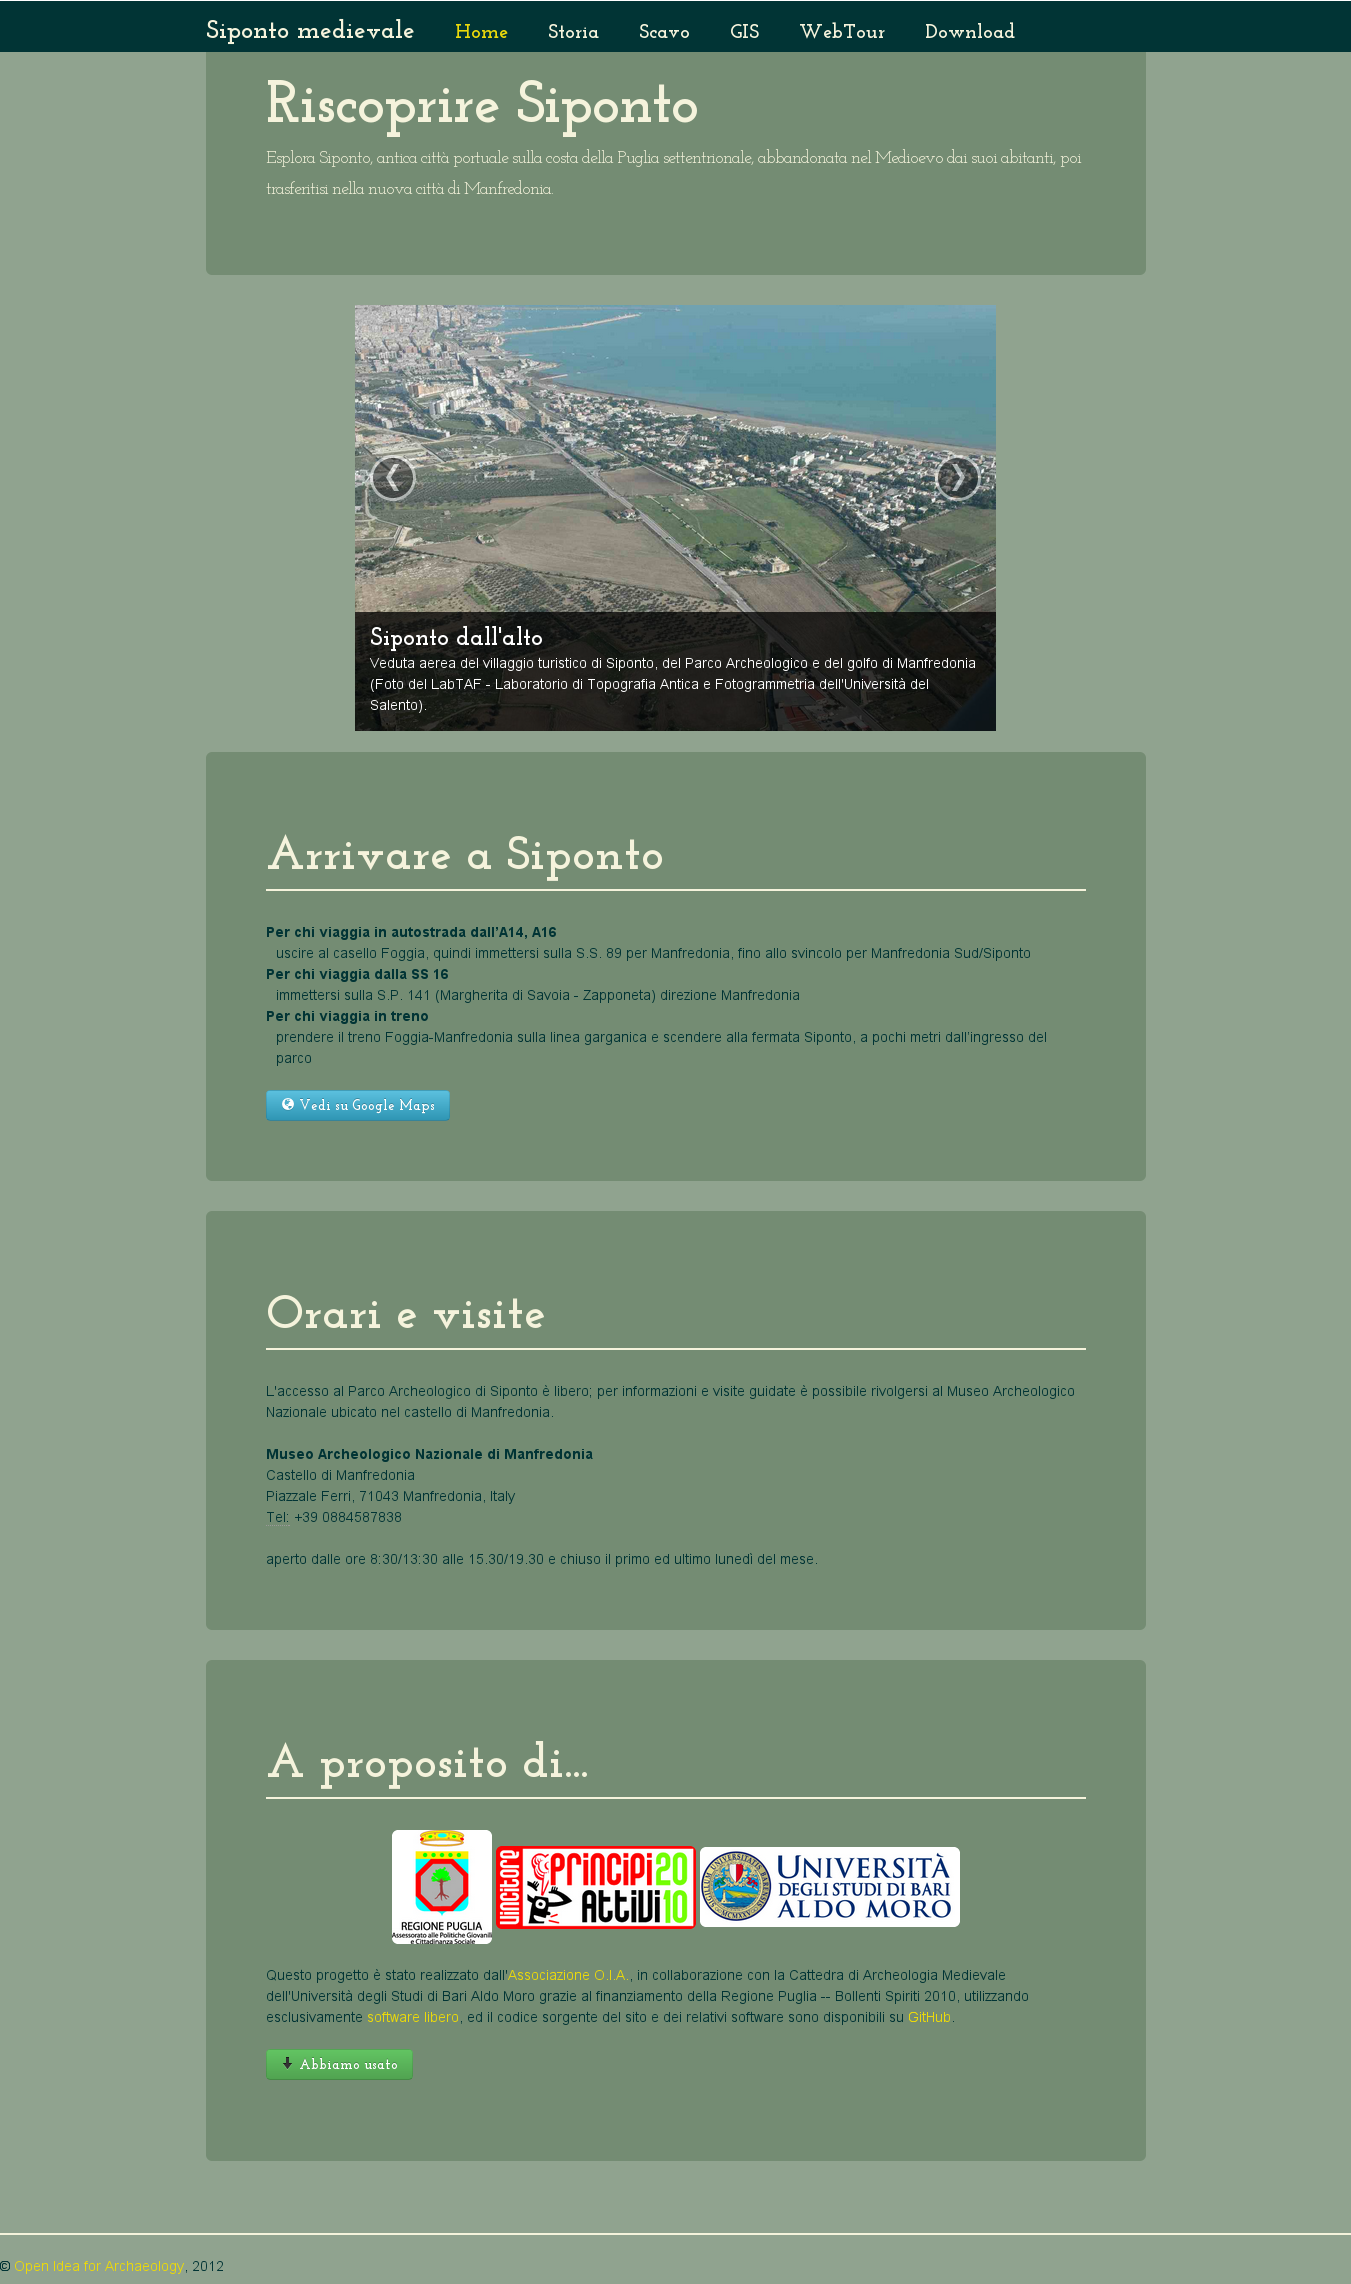
\includegraphics[width=0.8\textwidth]{img/home}
        \caption[\textit{Home page} di Siponto Aperta]{La \textit{Home Page} di Siponto Aperta.}
        \label{fig:home}
    \end{figure}

    \begin{figure}
        \centering
        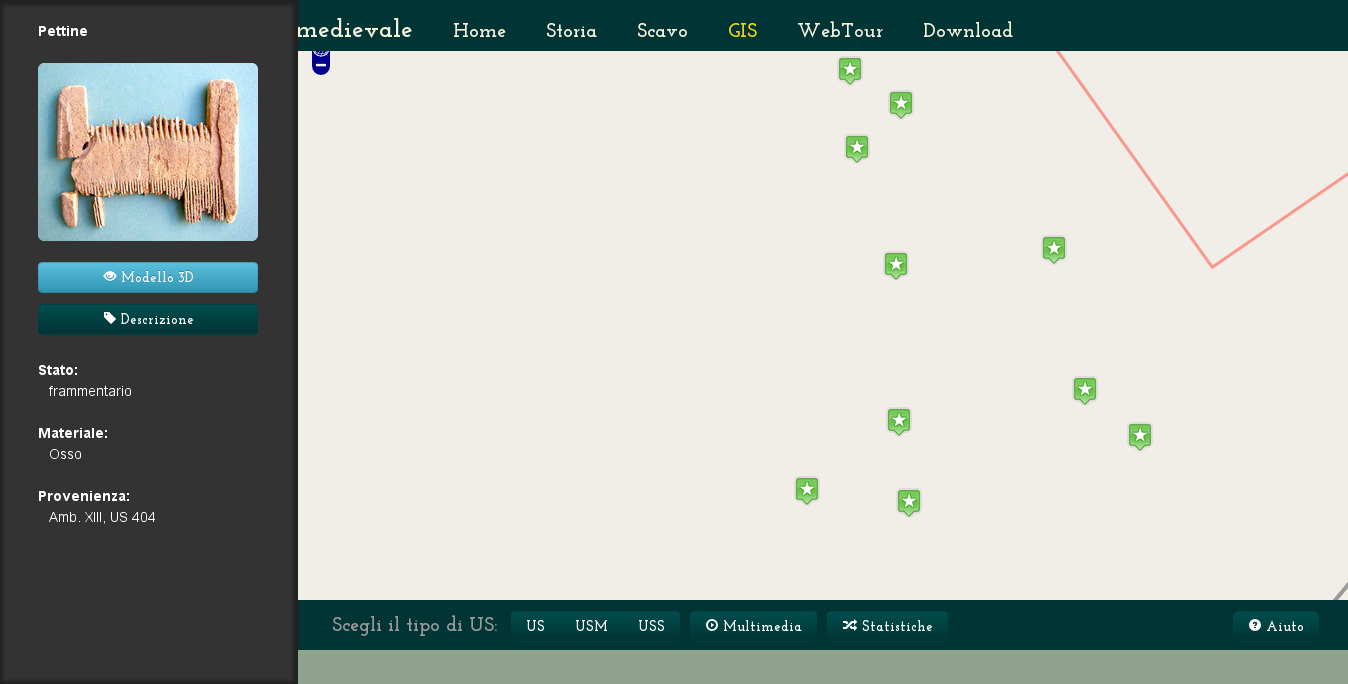
\includegraphics[width=0.8\textwidth]{img/gis}
        \caption[La pagina \emph{GIS}]{La pagina \emph{GIS}, in cui è aperta la scheda di un reperto ceramico dal layer multimediale.}
        \label{fig:gis}
    \end{figure}


\addcontentsline{toc}{section}{\refname}
\printbibliography

\end{document}
